\documentclass[12pt]{article}
\usepackage[margin=1in]{geometry} 
\usepackage{amsmath,amsthm,amssymb, graphicx, multicol, array}
\usepackage{mdframed}
\usepackage{enumerate}
\usepackage{pgf,tikz}
\usepackage{mathrsfs}
\usepackage{tikzscale}
\usepackage{pgfplots}
\usepackage[hidelinks]{hyperref}
\pgfplotsset{compat=newest}
%% the following commands are needed for some matlab2tikz features
\usepackage{grffile}
\usepackage{amsmath}
\usepackage{ulem}
%% you may also want the following commands

\newcommand{\N}{\mathbb{N}}
\newcommand{\Z}{\mathbb{Z}}
\newcommand{\Var}{\ensuremath{\text{Var}}}
\newcommand{\Cov}{\ensuremath{\text{Cov}}}
\newcommand{\Corr}{\ensuremath{\text{Corr}}}

\newcommand{\thetahat}{\widehat{\theta}}
\newcommand{\betahat}{\widehat{\beta}}
\newcommand{\yhat}{\widehat{y}}
\newcommand{\eps}{\varepsilon}
\newcommand{\xtilde}{\widetilde{x}}
\newcommand{\ytilde}{\widetilde{y}}
\newcommand{\ztilde}{\widetilde{z}}

\newtheorem{theorem}{Claim}
\newtheorem*{Claim}{Claim}
\newtheorem*{Definition}{Definition}


\begin{document}
	
	\title{Two sided labor market search\\The Diamond-Mortensen-Pissarides (DMP) model}
	\author{ECON 331}
	\date{}
	\maketitle
	


	
	
This set of notes outlines a different approach to the two-sided labor market (DMP) labor search model than the Williamson textbook.   Although the model has a some complicated microeconomics behind it, it will (eventually) result in a nice, graphical representation that we can easily use to compare steady states, which is our main focus.  It is based on the first chapter of \textit{Equilibrium Unemployment Theory,} second edition, by Christopher Pissarides.


\paragraph{The basic setup of the model} Workers can either be employed at a wage $w$, or unemployed.  Either state is persistent but can change. The probability of exogenously separating from your job is $\delta$.  We define (maximum) value functions for workers in either state: the value function for employed workers is $W$ and the value function for unemployed workers is $U$. 

Assume that the flow benefit of being employed in a period is the wage $w$, and the unemployment benefit  -- the value you get each period you're unemployed --  is $b$.

There are also firms in the model.  To operate, a firm must hire a worker.  Before it can hire, it has to  ``post a vacancy'' --  create the position and spend resources to actively recruit.  A firm that hires a worker (``fills'' the vacancy) starts producing the next period.  The value function of a firm with a filled vacancy is $J$; an unfilled vacancy has value function $V$.  Firms can also shut down and earn 0.  

A firm that hires a worker earns real revenue $z$ (think of this as the productivity of the worker) and must pay the wage $w$, so real flow profits are $z - w$.  If a firm wants to post a vacancy, it has to pay a fixed cost $k$.  (You could think about this cost as costs of conducing a search, interviewing candidates, and so on).

Assume that all the agents in the economy are risk neutral. This means when evaluating payoffs, they focus solely on expected financial value. We assume there is a (fixed, exogenous) real interest rate $r$; the discount rate for payoffs is  $\beta = \frac{1}{1+r}$.

\paragraph{The matching function} Rather than explicitly model how matches occur, we will use a ``matching function'' that describes the output (successful matches/new jobs) created from a given amount of inputs (firms with vacancies and searching workers).

%We will assume the matching function has the same properties Williamson does in his textbook, but adjust the notation.

Assume there are $u$ unemployed workers searching and $v$ unfilled vacancies.\footnote{This is a slight change of notation from the textbook, which uses $\mathcal{Q} = u$ and $A = v$.} The number of matches is $M = e \cdot m(u,v)$.  $m(u,v)$ is a constant returns to scale matching function that tells us how many matches occur for a given number of unemployed workers $u$ and employed workers $v$.   $e$ is a matching efficiency parameter. When $e$ is higher, all else equal, there are more matches (analogous to total factor productivity in a firm's production function).  We define $\theta = \frac{v}{u}$ \textbf{labor market tightness}. A very tight labor market is one where there are more job openings per worker.\footnote{In the Williamson textbook,  ``$j$'' is the symbol for labor market tightness, but $\theta$ is standard notation in this literature so that's what I use.}

All vacancies and workers are the same. Any given searching worker could randomly match up with any given vacancy with equal probability (and vice versa). That means that the probability that any \textit{given} vacancy is filled is just $M/v = \frac{e m(u,v)}{v} = em(u/v, v/v) = em(1/\theta,1)$ (where to rewrite it in terms of market tightness, we're using the assumption that the matching function is CRS). $em(1,\theta)$ is the probability an unemployed worker is matched (for similar reasons).  

\paragraph{Value equations} We write each matching function from the perspective of the end of a period.  The firm/worker knows which state they're in the next period and hence what their flow value for the next period is.  However, for the period after that, they have to form expectations.  We assume they do so using model-consistent (\textit{rational}) expectations; they know the true probabilities of transitioning between states and form expectations based on the correct expected value.  

A worker who starts the next period unemployed successfully matches after searching with probability $em(1,\theta)$. Workers do not start working until the period \textit{after} they match.  A worker who starts the period employed is separated with probaility $\delta$.  

The value equations for the worker, given her state of employment or unemployment today and the wage she is employed at, if employed:

\begin{eqnarray*}
	W = \beta w + \beta ((1-\delta) W + \delta U ) \\
	U = \beta b + \beta ( em(1,\theta) W + (1- em(1,\theta)) U)  \\
\end{eqnarray*}



A firm with a worker earns flow profits $z - w$.  To post a vacancy, the firm has to pay $k$.  After posting a vacancy, the firm matches with a worker with probability $em(1/\theta,1)$. 

So the value equations for the \textit{firm}:
\begin{eqnarray*}
J = \beta (z - w) + \beta ((1-\delta) J + \delta V)  \\
V = \beta (-k) + \beta (em(1/\theta,1) J + (1- em(1/\theta,1)) V)  
\end{eqnarray*}


% 


Since $\beta = 1/(1+r)$,  $1/\beta - 1 = r$.  Substituting for $\beta$ and re-arranging the above expressions, we can show that

\begin{equation}\label{eq:W}
	\begin{aligned}
		&W = \beta(w + (1-\delta) W  + \delta U ) & \\ \Rightarrow & r W = w + \delta [U - W]&
	\end{aligned}
\end{equation}

and similarly for the other expressions:


\begin{equation}\label{eq:U}
	\begin{aligned}
		r U  = b + e \cdot m(1, \theta) (W - U) 
	\end{aligned}
\end{equation}
\begin{equation}\label{eq:J}
	\begin{aligned}
		r J = (z - w) + \delta (V - J)
	\end{aligned}
\end{equation}
\begin{equation}\label{eq:V}
	\begin{aligned}
		r V = - k + e \cdot m(1/\theta, 1) (J - V)
	\end{aligned}
\end{equation}

Why do we have $r$ times the value on the left hand side? This is related to the present value of being employed.   In this model, each state of the world is like owning a financial asset that pays a fixed amount every period.  A financial instrument with this structure is called an \textit{annuity}.  For instance, being unemployed gives a fixed payment $b$ every period you're unemployed, plus whatever the expected value of searching is.  If we treat that payment as a flow value of unemployment, then the present value of that flow is $$U = \text{Present value of unemployed state} = \frac{\text{flow value of unemployment and expected gain}}{r}$$ 

(This is where risk neutrality comes in handy as an assumption, because we don't need to worry about how agents value the riskiness of search, just the financial payoff).

\paragraph{Defining the steady state equilibrium} We're going to focus on steady states.  In the steady state, we will assume that wages and market tightness turn out to be constant (and verify that this assumption is sensible).

Right now, we have four equations -- equations (1) - (4) and \textit{six} unknowns -- $W,U, J, V, \theta, w$.% (That is, the values of being employed and unemployed workers, and the value of a firm with and without a worker,  as well as the steady-state wage and market tightness).

Let's formally define the equilibrium concept for this extended model:

\begin{Definition}[Steady state equilibrium in the DMP model]
	A steady state equilibrium is a set of value functions $W,U,V,J$, market tightness $\theta$, vacancies $v$, number of unemployed workers $u$ and a wage $w $ such that, given a matching function $em(u,v)$, productivity $z$, discount rate $\beta = (1/(1+r))$, exogenous job destruction probability $\delta$, flow rate of unemployment $b$, and defining market tightness $\theta \equiv v/u$:
	\begin{enumerate}
		\item Households optimally choose to search for work, given their probability of finding a job $em(1,\theta)$ and the rate of job destruction $\delta$, the flow benefit of unemployment $b$, taking as given the wage determination process;
		\item Firms optimally choose to post vacancies, given the cost of posting $k$, the probability of filling a vacancy $em(1/\theta,1)$ and the rate of job destruction $\delta$, and taking as given the productivity of workers $z$ and the wage determination process;
		\item There is free entry by firms;
		\item Wages are determined by bilateral Nash bargaining;
		\item The unemployment rate is constant.
	\end{enumerate}

\end{Definition}

You may be looking at this definition and not be sure where to begin. That is totally okay. There are a lot of moving parts, and this theory was worked out, over time, by people who literally won a Nobel Prize for doing it.

To solve the model, we'll use the last three conditions: free entry, Nash bargaining, and then a constant unemployment rate.

\subsection*{Free entry and the job creation curve}

The first important condition we'll impose is \textit{free entry}.  Firms are allowed to enter (and exit, by shutting down); there is no limit to how many firms \textit{could} exist, only an economic reason that a finite number of firms will choose to enter. Free entry pins down the equilibrium value of a vacancy.  If $V > 0 $, then it is beneficial (in a present value sense) for a firm to enter and post a vacancy.  Doing so, however, increases market tightness, which lowers the probability of filling a vacancy and hence the value of all vacancies, which lowers $V$.  Similarly, if $V < 0 $, firms would be better off exiting (and earning 0). This lowers market tightness and makes all vacancies more valuable (because they're more likely to be filled and produce profits).   The free entry and exit of firms drives the present value of a vacancy to 0:

\begin{equation}\label{eq:freeentry}
	\begin{aligned}
V = 0
	\end{aligned}
\end{equation}

We can use this free entry condition to derive a \textbf{job creation curve} -- a relationship between wages and market tightness that consistent with firms' optimal decision to enter. Combine \eqref{eq:freeentry} with \eqref{eq:V} and solve for $J$:

\begin{equation*}
	\begin{aligned}
		&k = em(1/\theta,1)\times J &\\
		\Rightarrow &J = \frac{k}{em(1/\theta,1)}&
	\end{aligned}
\end{equation*}

The first line of the above says that the cost  of creating a vacancy must be equal to its expected benefit (the probability of filling it times the present value of a filled vacancy).


Now, substitute this expression into \eqref{eq:J} to relate market tightness to \textit{wages} (also substituting $V = 0$)

\begin{equation*}
	\begin{aligned}
			&	r J = (z - w) + \delta (V - J) &\\
			\Rightarrow& (r+\delta) J = (z-w) &\\
			\Rightarrow &w = z - \frac{k}{em(1/\theta,1)} (r + \delta)
	\end{aligned}
\end{equation*}

Rewriting slightly:

\begin{equation}\label{eq:JC}
		w = z - (r + \delta) \frac{k}{em(1/\theta,1)} \tag{JC}
\end{equation}

This is the equation for the Job Creation (JC) curve.  It summarizes the optimal behavior of firms, consistent with their free entry condition.  It says that, in equilibrium, wages are positive related to productivity ($z$) less the an adjusted cost of creating the vacancy.

Note that firms earn positive (flow) profits here; in general $w < z$.  Because the wage is less than workers' productivity, the firm keeps a little more than what the workers' output sells for.  Firms must earn positive profits once they've filled a vacancy to cover the fixed cost of posting the vacancy initially.  

If we plot this curve (figure \ref{fig:JC}) it's downward-sloping; higher $\theta$ means a lower probability of filling a vacancy, which means we're dividing by a smaller number in the negative term.  The precise shape of the $JC$ curve is going to change depending on the curvature of the $m(u,v)$ function. 




\begin{figure}
\begin{center}
	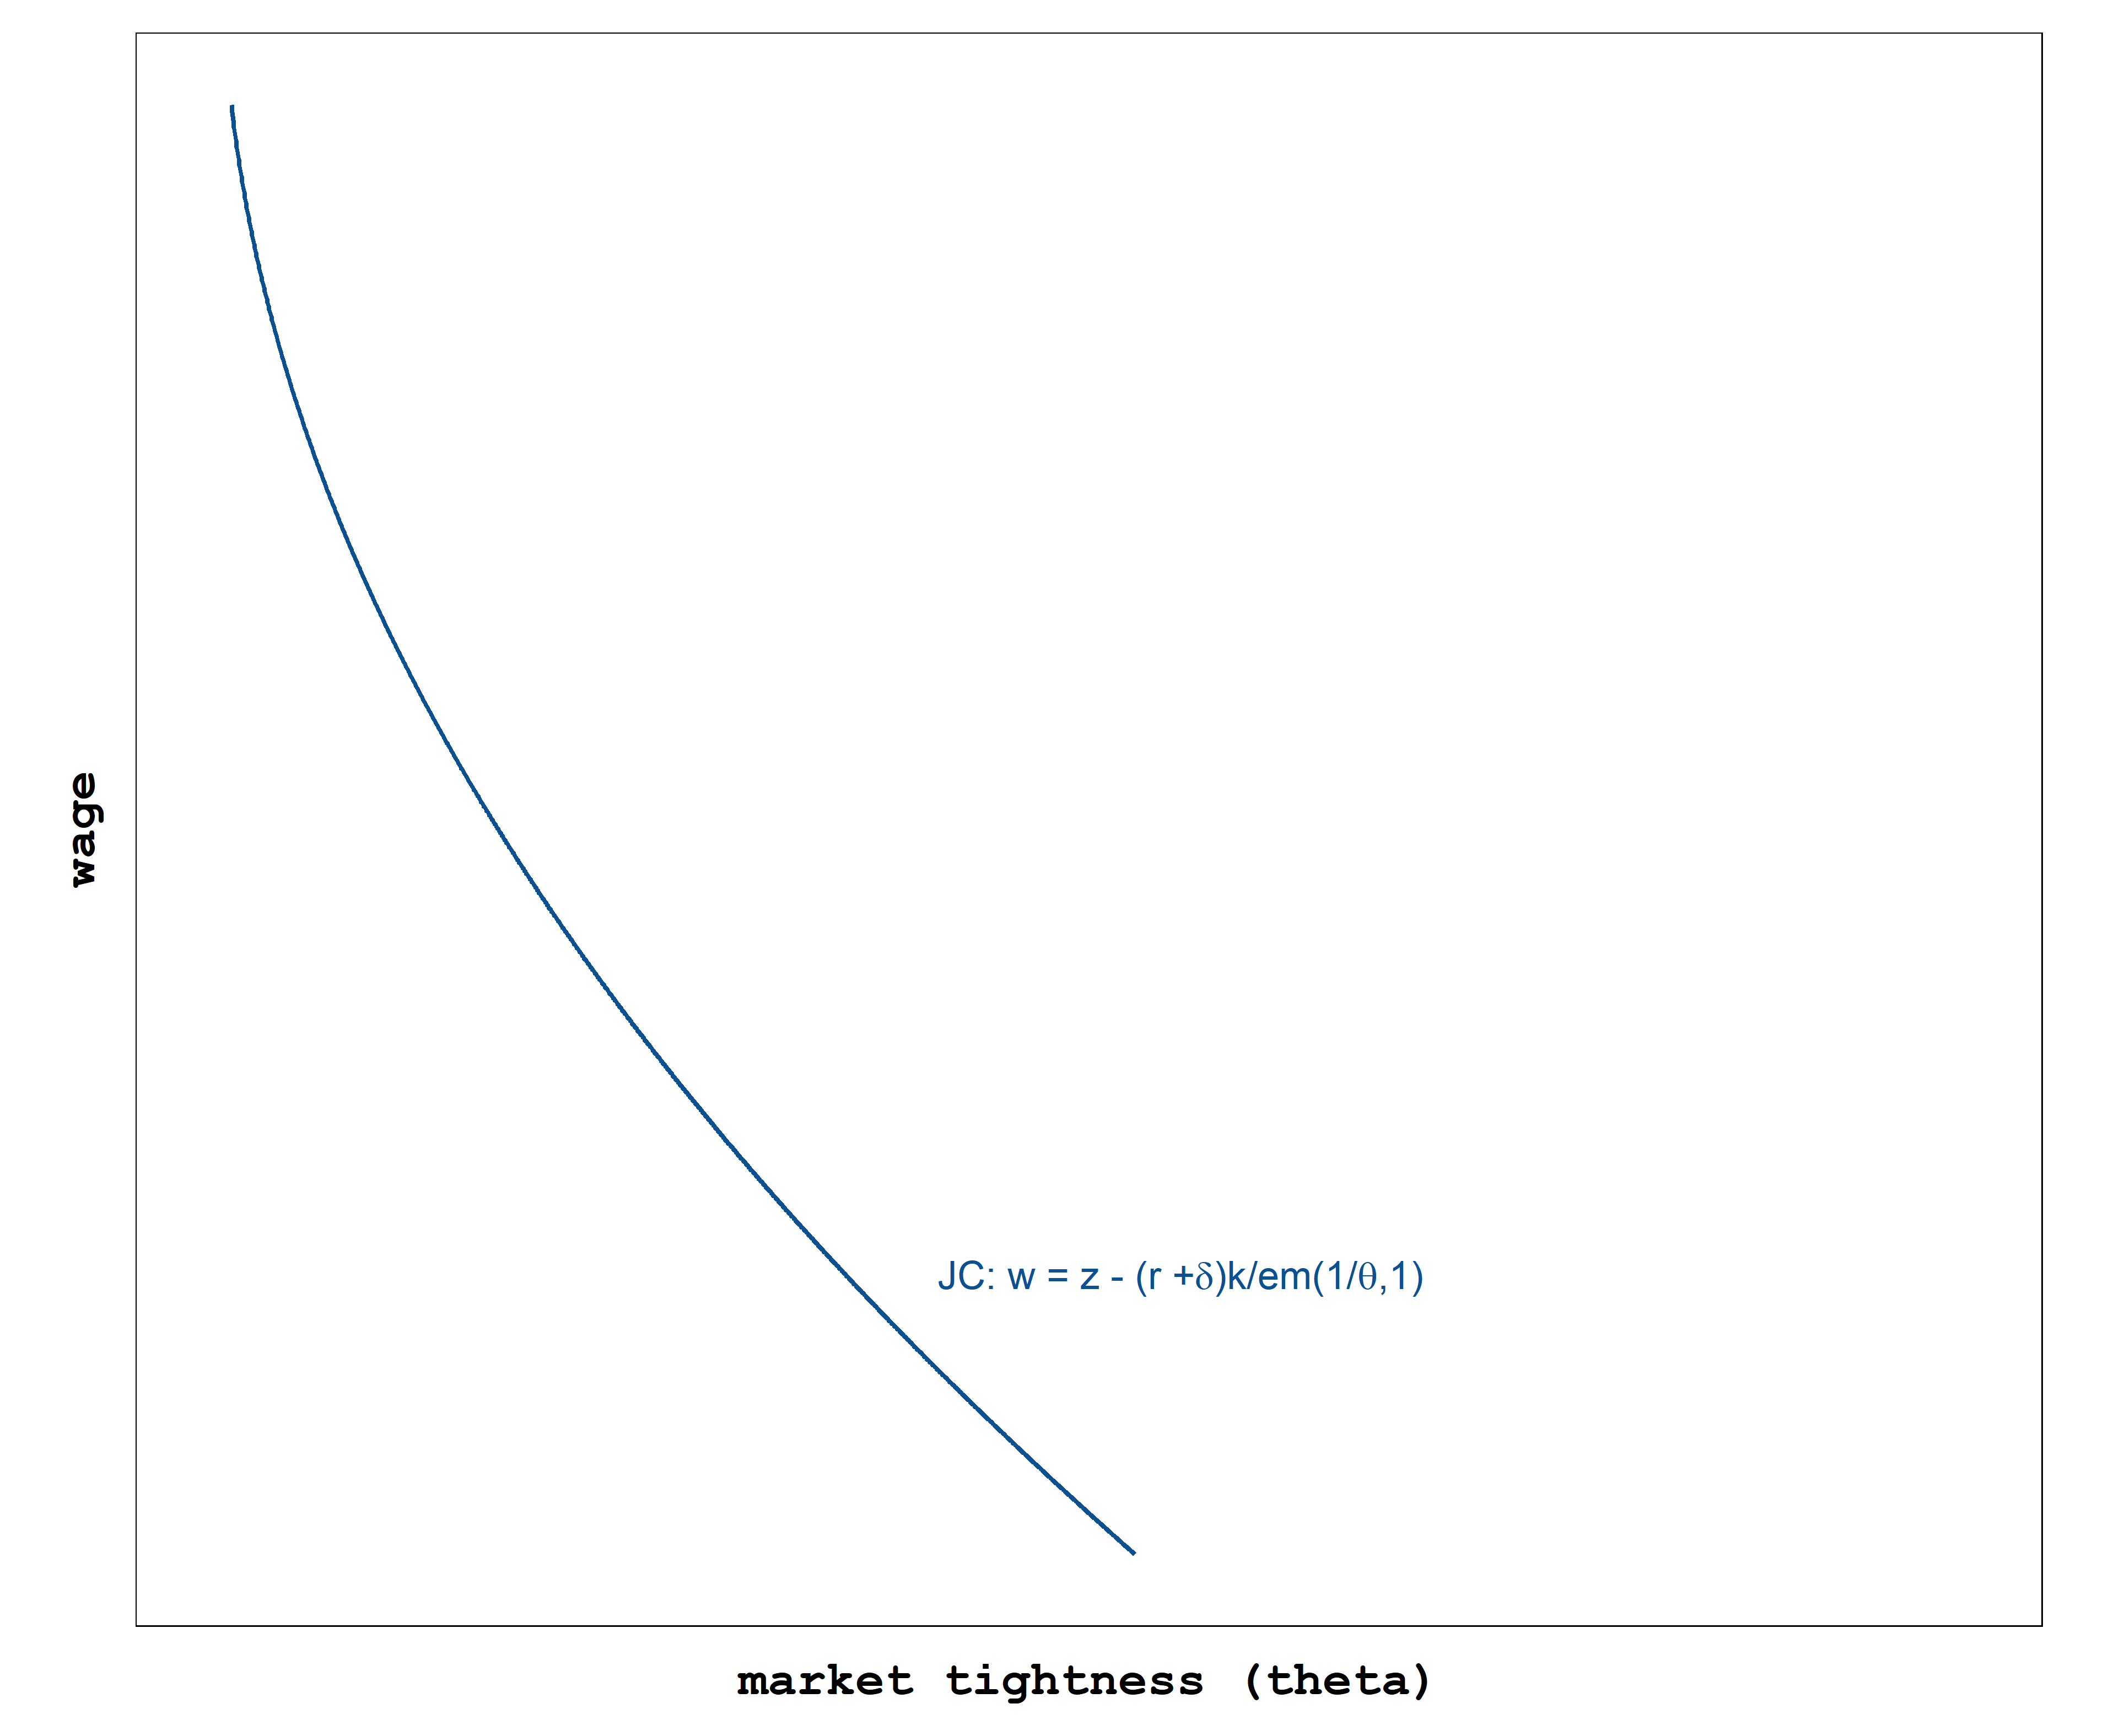
\includegraphics[height = .33\textheight]{jc.png}
\end{center}
\caption{The JC curve.  The free entry condition pins down the equilibrium value of a vacancy, which in turn summarizes the firm's optimal vacancy posting condition in terms of wages and market tightness.}\label{fig:JC}
\end{figure}

This curve shifts to the right (a higher level of market tightness for a given wage) if $z$ or $e$ increase, or if $r, \delta$ or $k$ fall.  A change in $\theta$ is a movement along the curve.  The economic interpretation of these changes are (hopefully) intuitive:
\begin{itemize}
	\item  A higher $z$ means any given job is worth more to the firm at a given wage.  That increase the incentives to post vacancies.
	\item A lower $\delta$ means that any given match is expected to last a longer time, increasing the benefit of vacancy posting for the firm (because you won't have to pay the vacancy posting cost very often).
	\item Lower vacancy posting costs $k$ mean the net benefit of posting a vacancy is higher at a given wage
	\item A higher $r$ means that the rate at which firms discount the future is greater, lowering the present value of posting a job from the firm's point of view. 
\end{itemize} 

\subsection*{Nash bargaining and the ``Wage curve''}

We will assume that wages are determined by bargaining  once a worker matches with the firm. How do they bargain? The common assumption in this literature is \textit{bilateral Nash bargaining}.  The household and the firm attempt maximize the \textit{joint} surplus of a successful match -- the total benefit of matching relative to both receiving the outside option -- and then they divide it up.  We assume that the worker and the firm each have different (relative) bargaining power determined by the parameter $a$.  $a$ is the bargaining power of workers, $1-a$ is the bargaining power of firms.

Showing this fact involves two tedious derivations.  I've moved them to an appendix at the end of this set of notes for the sake of clarity, and instead I will give you the setup and punchline.

First, note that the value of a filled vacancy for the worker and firm depends directly on $w$ so we can explicitly write the bargaining problem as a choice of $w$ to maximize the product of the surplus created by filling the match:

$$ \max_w [(W(w) - U)^a \times (J(w) - V)^{1-a}] $$

 $W - U$ is how much the worker gains by accepting the job instead of remaining unemployed (her outside option); $J - V$ is the gain of the firm for hiring rather than having an open vacancy.




\begin{theorem} \label{claim1}
Call the total surplus $J + W - U$, where we've used the fact that $ V= 0$.  The Nash bargaining solution implies that the worker receives  a constant fraction $a$ of the total surplus, so $W-U = a (J  + W - U)$.  The firm receives  $J = (1-a)(J + W -U)$

\end{theorem}

\begin{proof} 
See section \ref{claim1proof} in the math appendix.
\end{proof}


From here, we substitute out the value functions in the Nash bargaining solution in order to once again find an expression for $w$ in terms of market tightness $\theta$ and parameters.  





The next set of steps is a little esoteric. We need to get rid of the value equations to find an expression for $w$ in terms of parameters and $\theta$.  To do that, we start with our value equations. \eqref{eq:W}, solving for $W$, implies that

$$ W = \frac{w}{r + \delta} + \frac{\delta}{r + \delta} U $$

and $\eqref{eq:J}$, solving for $J$, gives us that

$$ J = \frac{z - w}{r + \delta} $$

Substituting these into the Nash bargaining solution and a lot of tedious algebra leads to the following expression

\begin{theorem}\label{claim2}

Nash bargaining implies the following expression, the ``wage curve'', which represents wages that satisfy Nash bargaining at a given level of market tightness.

\begin{equation}\label{eq:WC}
	w = b + a (z - b +  k \theta) \tag{WC}
\end{equation}

\end{theorem}
\begin{proof}
See math appendix \ref{claim2proof}.
\end{proof}


We'll call this the ``Wage Curve'' (WC).  It's shown in figure \ref{fig:WC}. This expression relates wages to market tightness consistent with the equilibrium outcome of the Nash bargaining process.  This wage curve is really a wage \textit{line} with constant slope $a k$.  It tells us that wages must give workers not just the value of their outside option of being unemployed but will also compensate them for their productivity and the gain firms enjoy for not having to pay hiring costs in the future.  Market tightness impacts the wage positively according to this condition; tighter labor markets mean that a searching worker will very likely find a job which improves their bargaining position; They can credibly threaten to walk away from the bargaining table, knowing they will quickly find a new job.

This curve is shifted upward (a higher wage at a given market tightness) if $b$, $z$, or $k$ increase.  Since this is a linear equation, it's easy to see that an increase in productivity by $\Delta z$ will shift this curve upward by $a \Delta z$, or less than the change in productivity, because productivity improvements only partially pass through to wages. A similar argument holds for the other changes.  

\begin{figure}
\begin{center}
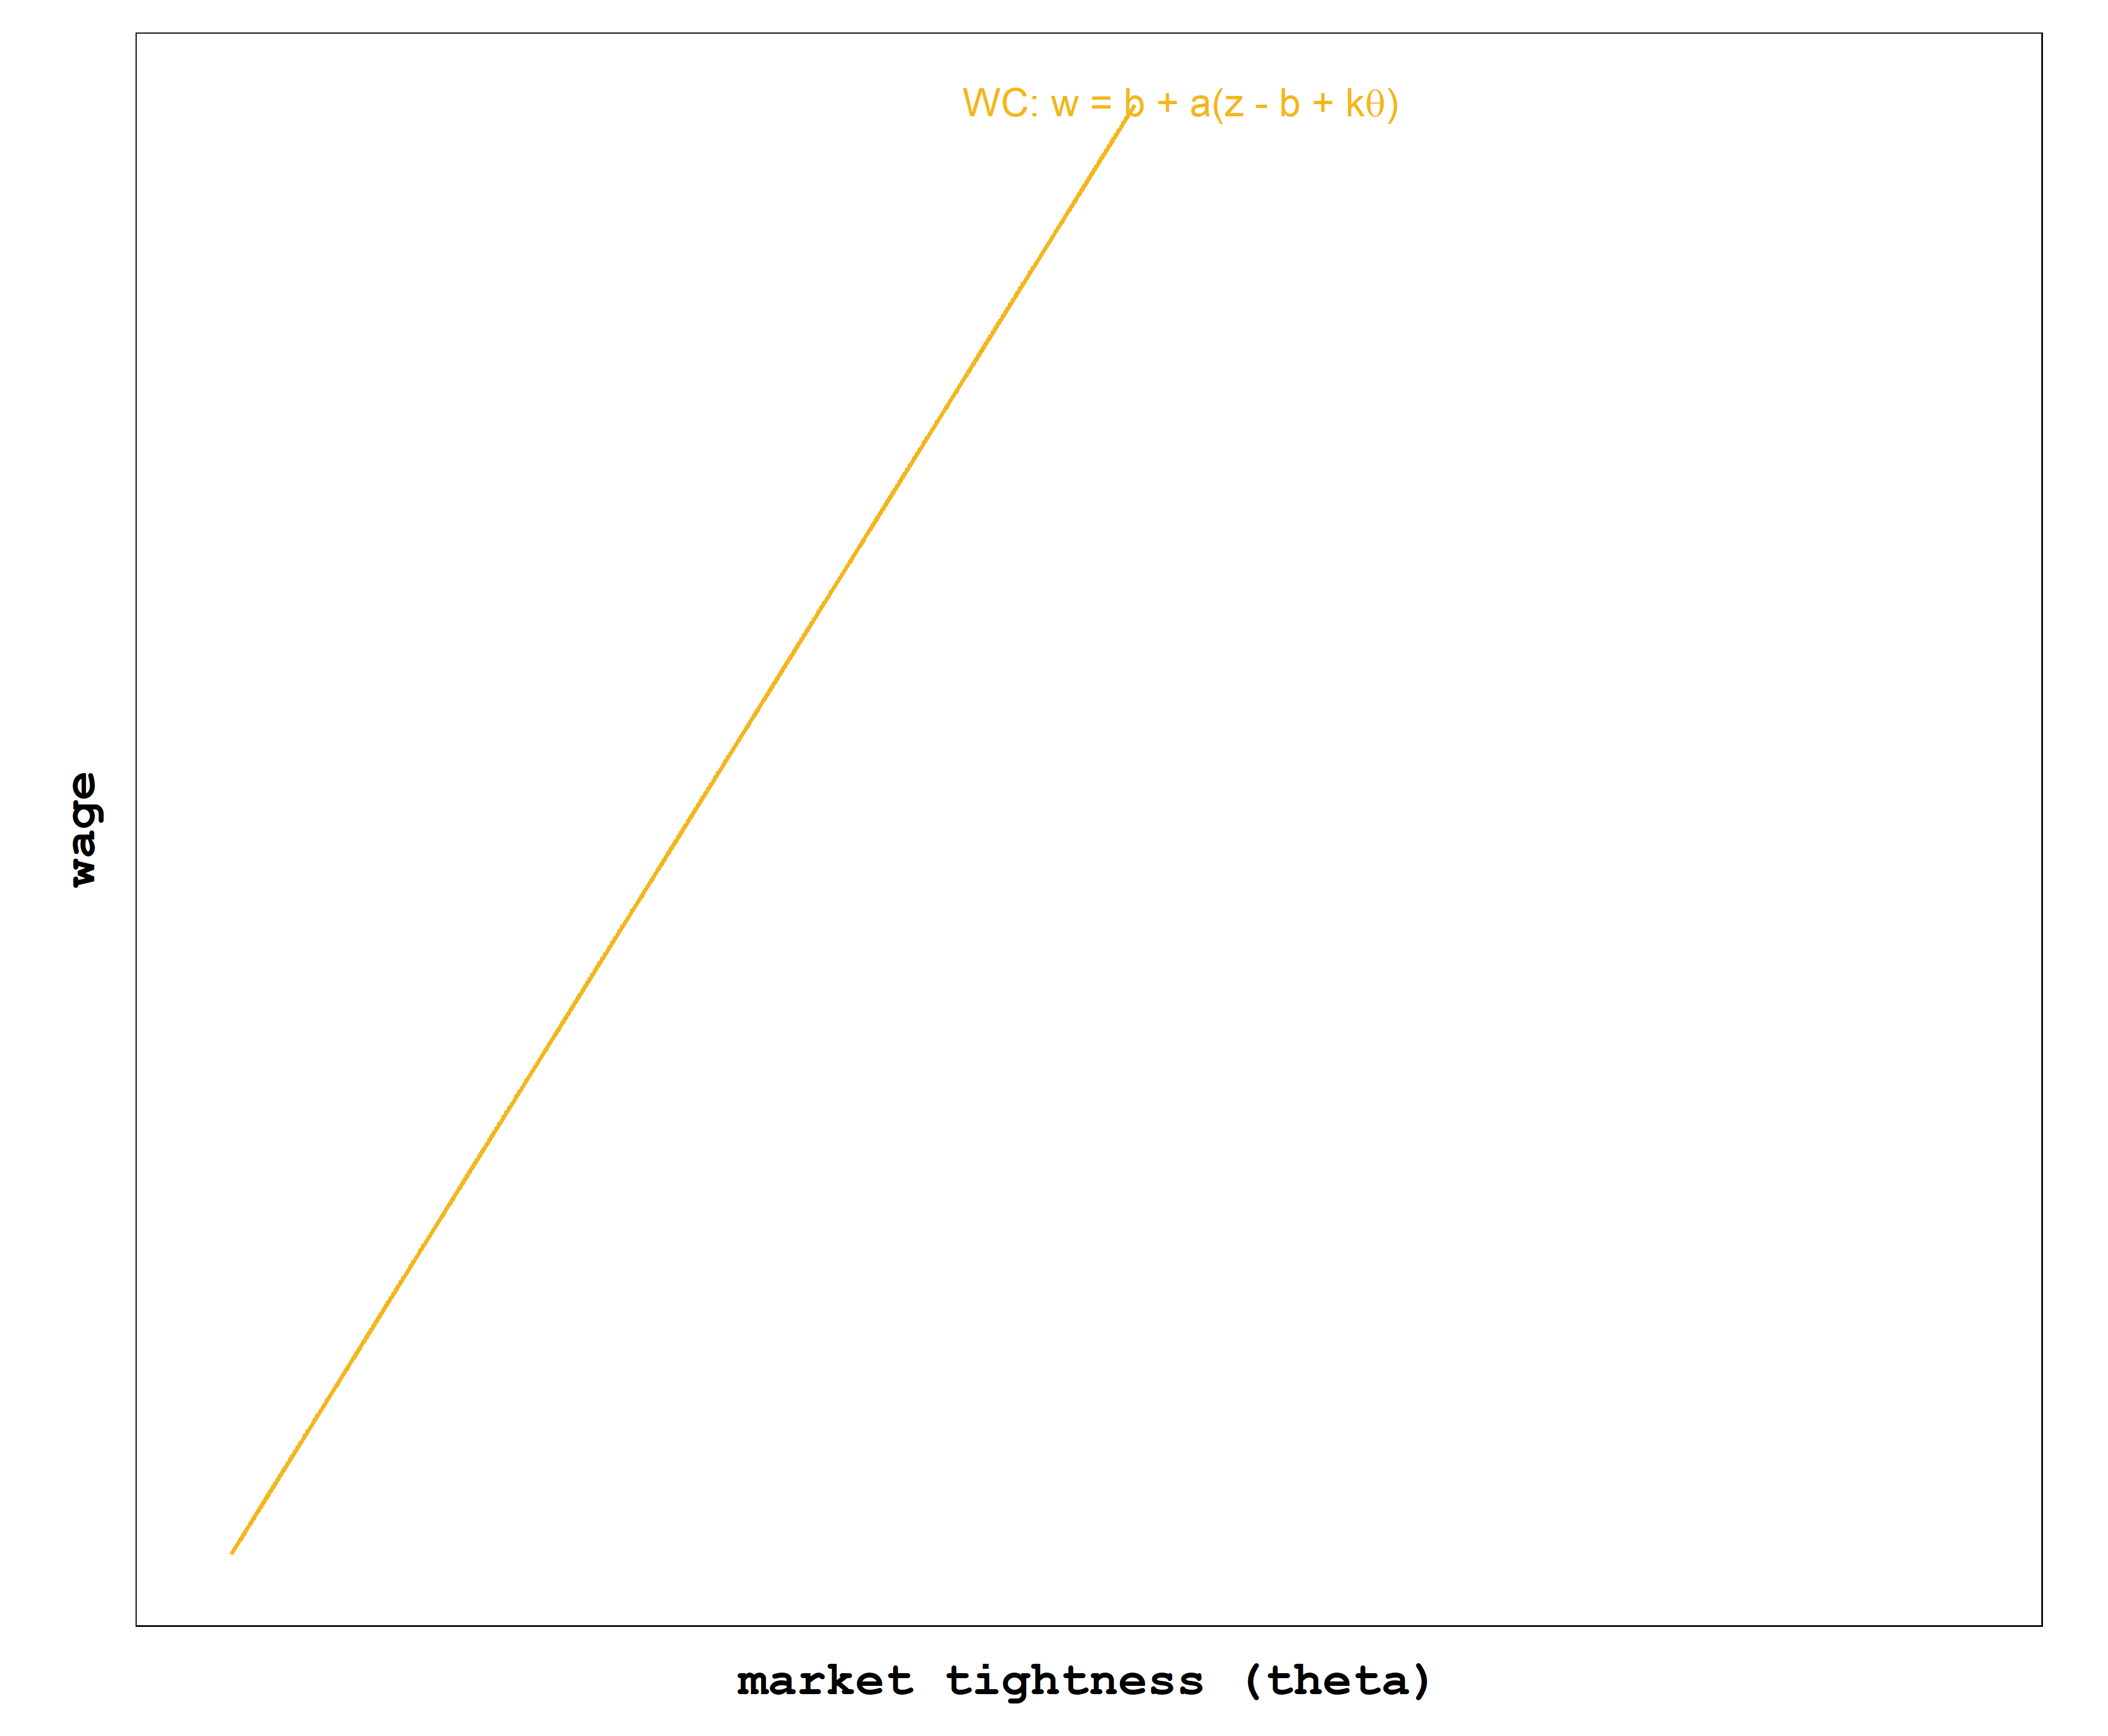
\includegraphics[height = .33\textheight]{wc.png}
\end{center}
\caption{The WC curve.  Nash bargaining determines the combinations of wages and market tightness consistent with the optimal behavior of households and firms, resulting in the linear WC schedule.  Yes, WC curve is redundant, like ATM machine.}\label{fig:WC}
\end{figure}

\subsection*{Equilibrium and solving for the unemployment and vacancy rates}

We can solve for the wage and market tightness by finding the intersection of the two curves, which summarize the optimal behavior of firms and workers (figure \ref{fig:wcjc}).

\begin{figure}[htb]
\begin{center}
	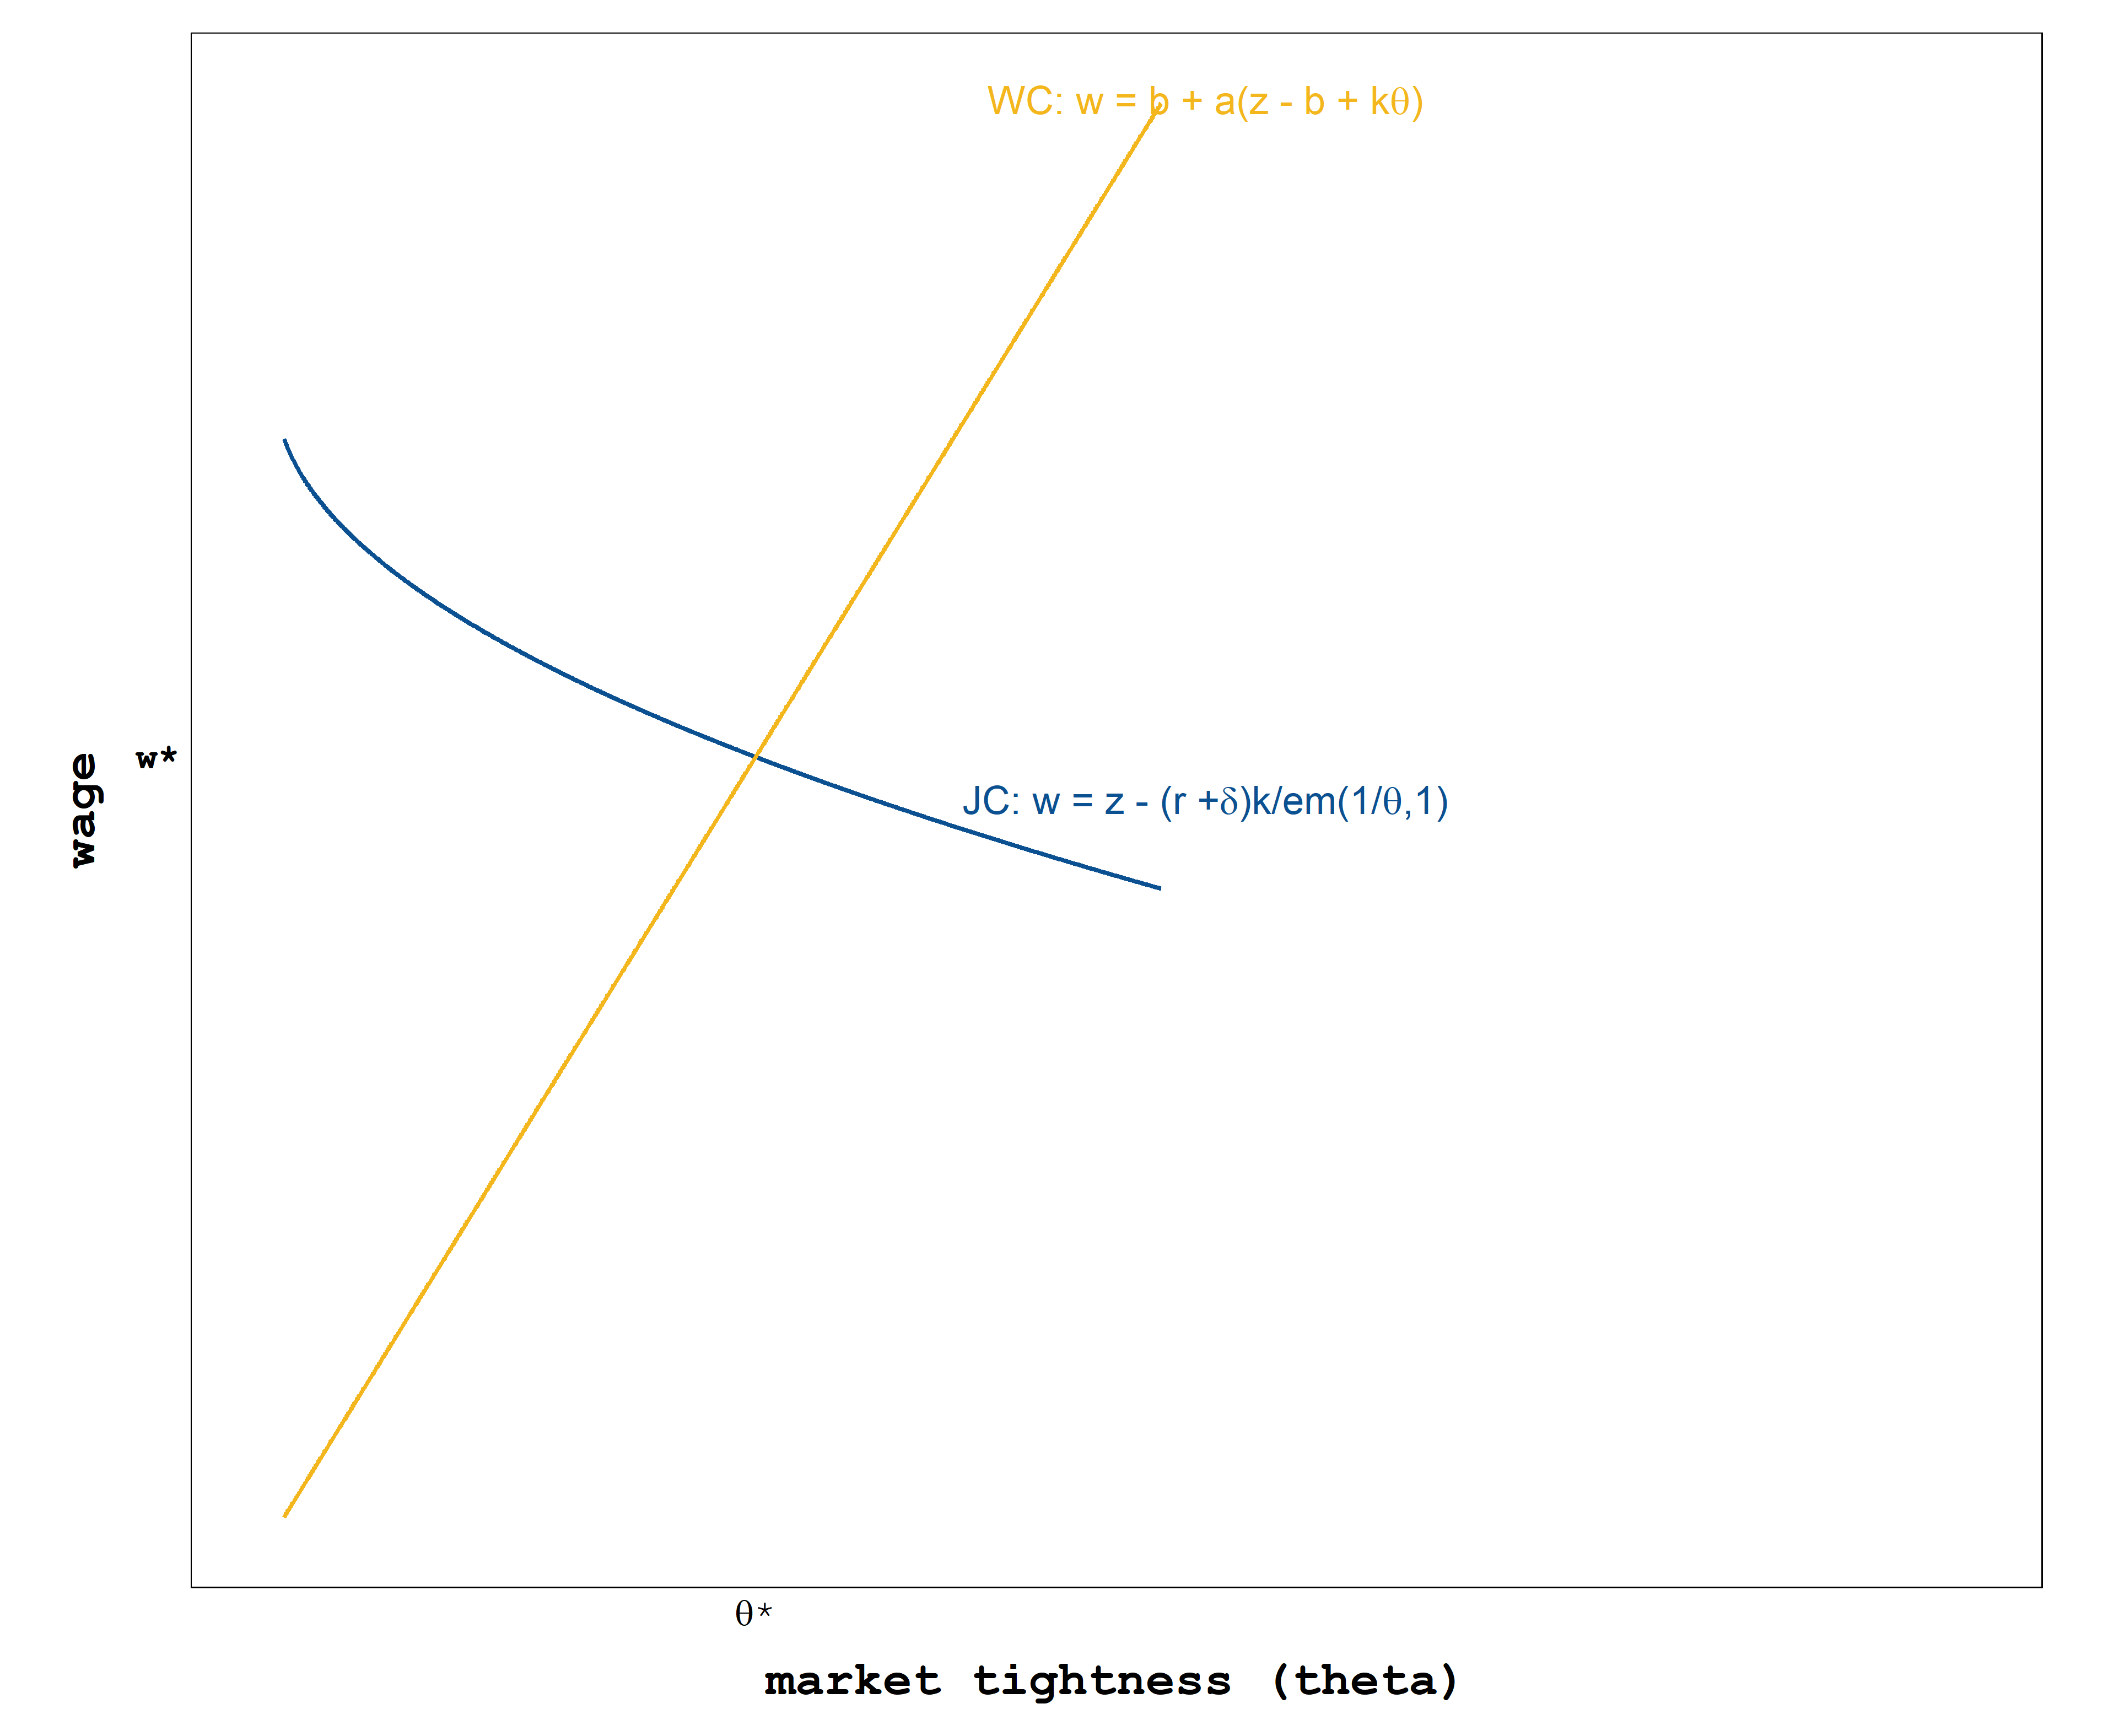
\includegraphics[height = .33\textheight]{eqm_wj.png}
\end{center}
\caption{The equilibrium wage and market tightness is determined by the intersection of the JC and WC schedules.}\label{fig:wcjc}
\end{figure}

On some level, it may look like we've got an upward sloping supply and downward sloping demand.  But the intersection of these two curves does \textit{not clear} the market, and it \textit{does not} set wages equal to marginal productivity.  Workers are paid less than their marginal product, but more than the minimum that would be required to induce work. Firms earn positive profits, and some workers and firms do not manage to find one another in steady state.

What {is} the unemployment rate? We only know $\theta$ and $w$.  In fact, solving for the equilibrium level of market tightness (setting \eqref{eq:JC} and \eqref{eq:WC} equal to one another)

$$z - b = \frac{1}{1-a} \left[ \frac{(r + \delta )k}{em(1/\theta,1)} + a k \theta  \right] $$

This \textit{implicitly} defines market tightness in terms of the parameters of the model, but is silent on the actual number of vacancies or unemployed workers.  However, we know that in steady state, the unemployment rate must be constant.  This means that any worker being fired is offset by a worker that is being matched to a new firm. If there are $E$ total employed workers and total unemployed workers of $Q$, then

$$\delta E = em(1,\theta)Q$$

The unemployment $rate$ is $Q/(Q+E)$.  Re-arranging the previous equation to solve for for $Q$ in terms of $E$ and then plugging that into the definition of the unemployment rate gives that

\begin{equation}\label{eq:bev}
	u = \frac{\delta}{\delta + em(1,\theta)} \tag{Beveridge Curve}
\end{equation}

This is the model version of the Beveridge curve we saw in the data -- a negative relationship between market tightness and the unemployment rate.  It's curvature comes from the curvature of the matching function $m$.  It is shifted only by changes in the separation rate $\delta$ and matching efficiency $e$. 

Graphically, we find $u$ by plotting $\theta^*$ in a graph with $v$ on the vertical axis and $u$ on the horizontal axis (this will be a straight line out of the origin with slope $\theta^*$).  We then plot the Beveridge curve; their intersection determines the precise quantity of $u$ and $v$ in equilibrium, as shown in figure \ref{fig:equv}.  (Since nothing in this graph would be changed by multiplying by the size of the labor force, finding the number of unemployed is equivalent to finding the unemployment rate in this model).

\begin{figure}[htb]
\begin{center}
	\includegraphics[height = .33\textheight]{Bev.png}
\end{center}
\caption{The Beveridge curve, combined with equilibrium market tightness, determines the steady-state level of unemployment and vacancies.}\label{fig:equv}
\end{figure}


\subsection*{Summing up}

The DMP model ultimately boils down to solving for the JC curve, the WC relation, and then their intersection to pin down market tightness and the wage.  Then, we can find where $\theta^*$ falls on the Beveridge curve to find the quantity of vacancies and unemployment. 

There are a number of exogenous variables in the model: $b, z, k, r, \delta, e$ in particular.  We might be interested in understanding how the different shifts correspond to different levels of market tightness, wages, and unemployment in steady state.  (We could also examine changes in bargaining power, which changes both the slope and intercept of the WC condition!).  We'll practice this in class.


\newpage
\appendix
\section{Math appendix}
\subsection{Proof of claim \ref{claim1}}\label{claim1proof}



\begin{Claim}
Call the total surplus $J + W - U$, where we've used the fact that $ V= 0$.  The Nash bargaining solution implies that the worker receives  a constant fraction $a$ of the total surplus, so $W-U = a (J  + W - U)$.  The firm receives  $J = (1-a)(J + W -U)$
\end{Claim}


\begin{proof}
Remember the bargaining problem is:

$$ \max_w [(W(w) - U)^a \times (J(w) - V)^{1-a}] $$

The first order condition with respect to $w$ is

$$a(W - U)^{a-1} W^\prime(w)(J - V)^{1-a}+(W - U)^a \times (1-a)(J - V)^{-a} \times J^\prime(w) = 0 $$

We can simplify by multiplying through by $(W - U)^{1-a} (J - V)^a$

$$W^\prime(w) a(J - V) + J^\prime(w)(1-a)(W - U) = 0$$

We can substitute out for $W^\prime(w)$ and  $J^\prime(w)$  by taking the derivative of \eqref{eq:W} and \eqref{eq:J}, respectively. Doing so, we note that 

$W^\prime(w) = \frac{1}{r + \delta}$ and $J^\prime(w) = -\frac{1}{r+\delta}$.  In other words, $W^\prime = - J^{\prime}$.  This makes sense: at the optimum, the benefit of increasing the worker's wage is exactly offset by the cost to the firm.

Using that fact and and the fact that $V= 0$, the previous expression can be written

$$W^\prime(w) a (J - V) - W^\prime(w) (1-a) (W - U) = 0$$

which implies

$$a (J + W - U) = W - U $$

That is, the wage bargain results in the worker receiving a constant fraction $a$ of the total surplus $(J + W - U)$. Similarly, firms receive $J = (1-a)(J + W -U)$
\end{proof}

\subsection{Proof of Claim \ref{claim2}}\label{claim2proof}

\begin{Claim}

Nash bargaining implies the following expression, the ``wage curve'', which represents wages that satisfy Nash bargaining at a given level of market tightness.

\begin{equation}\label{eq:WC}
	w = b + a (z - b +  k \theta) \tag{WC}
\end{equation}

\end{Claim}


\begin{proof}
Starting from the Nash bargaining solution, we substitute in for $W$ and $J$ using \eqref{eq:W} and \eqref{eq:J}:

\begin{align*}
	W - U &= a (J + W - U) &  \\
\Rightarrow	\frac{w}{r + \delta} + \frac{\delta}{r + \delta} U - U &= a \left(\frac{z - w}{r + \delta}  + \frac{w}{r + \delta} + \frac{\delta}{r + \delta} U - U \right)&\\
\end{align*}





Since $\delta/(r + \delta) - 1 = -r/(r+\delta)$

\begin{align*}
	\frac{w}{r + \delta} - \frac{r}{r + \delta} U &= a \left(\frac{z - w}{r + \delta}  + \frac{w}{r + \delta}  - \frac{r}{r + \delta} U \right) &\\
\end{align*}

\begin{align}\label{eq:rU}
		w &= rU + a (z - r U) & \tag{$\star$}
\end{align}

where we've gone to the last line by multiplying by $r + \delta$ and simplifying.  

Note that $rU$ is the annuity value of the state of being unemployed.  The wage must pay at least as much as this value, plus some fraction of productivity created by the worker net of the value of this outside option. The amount of that fraction is related to how much bargaining power we assume the workers have.

We want to get rid of $rU$.   $\eqref{eq:U}$ tells us $rU$   in terms of $W - U$, so let's start there.   To find $W - U$: 
 
 The firm's share of the surplus is $J = (1-a) (J + W - U)$.  We know from free entry that  $V = 0$ so equation \eqref{eq:J} implies $J = \frac{k}{e \cdot m((1/\theta),1)}$ .    And we know from \eqref{eq:U} that $ (rU - b)/(em(1,\theta)) = W - U$.  Substituting both of these into the firm's share of the surplus: 
 
 
$$ \frac{k}{e  m((1/\theta),1)} = (1-a)  \left[\frac{k}{e  m((1/\theta),1)} + \frac{ (rU - b)}{(em(1,\theta))} \right]  $$


We want to solve this for $rU$.  To simplify this expression, note that  

$$ \frac{e m(1,\theta)}{e m(1/\theta,1)} = \frac{ m(u,v)/u}{m(u,v)/v} = \theta$$.   

so then (multiplying through by $em(1,\theta)$):

$$ \frac{a}{1-a} k \theta + b = rU$$

Plugging this in back into the expression \eqref{eq:rU}, we get

\begin{equation*}
	\begin{aligned}
		w = rU + a (z - r U) = (1-a) rU + a z = (1-a) \left[b + \frac{a}{1-a} k \theta \right]  + a z
	\end{aligned}
\end{equation*}
which, simplifying gives the desired expression:
\begin{equation*}
	w = b + a (z - b +  k \theta)
\end{equation*}

\end{proof}

\end{document}